\chapter{Технологический раздел}
В данном разделе производится выбор средств программной реализации метода распознавания спортивных действий человека на видео, описывается формат входных и выходных данных. Приводятся детали реализации программных компонентов, предоставляются результаты тестирование разработанного метода, описывается взаимодействие пользователя с интерфейсом ПО, реализующим метод.  
\section{Входные и выходные данные}

Входными данными является видео, на котором челочек выполняет фитнес упражнения. Видео может быть любого размера, вертикальное или горизонтальное, формата mp4. Видео должно быть с нормальным освещением и одним человеком в кадре.

Выходные данные -- название класса вида действия на видео, к которому оно относится с наибольшей вероятностью и видео сформированное из кадров, на которых изображены градиенты интенсивностей каждого пикселя.

\section{Выбор языка программирования}

В качестве языка реализации разрабатываемого метода был выбран
Python версии 3.11. Использование данного языка обусловлено тем, что он часто используется в области машинного
обучения и имеет доступную документацию и библиотеки данной предметной области.

В разработанном ПО были использованы следующие библиотеки и фреймворки:

\begin{itemize}
	\item[---]  Scikit-learn \cite{sklearn} является библиотекой для работы с машинным обучением. Была использована при реализации метода случайных лесов;
	\item[---]  OpenCV \cite{opencv} представляет собой библиотеку для
	работы с компьютерным зрением, обработки изображений и набором сопутствующих алгоритмов;
	\item[---]  Flask \cite{flask} представляет собой фреймворк для создания веб-приложений на языке программирования Python, использующий набор инструментов Werkzeug, а также шаблонизатор Jinja2;
	\item[---]  Scikit-image \cite{skimage} представляет собой библиотеку обработки изображений с открытым исходным кодом для языка программирования Python.
\end{itemize}


\section{Разработка ПО}

\subsubsection{Требования к разрабатываемому ПО}

ПО, предоставляющие интерфейс для разрабатываемого метода должно предоставлять:
\begin{itemize}
	\item[---] возможность загрузить видео формата mp4;
	\item[---] возможность просмотреть какие виды действий могут быть распознаны;
	\item[---] воспроизводить загруженное видео и видео с градиентами интенсивностей;
	\item[---] выводить предсказанный вид действия.	
\end{itemize}

На рисунке 3.1 представлена UML диаграмма вариантов использования разработанного ПО, доступные пользователю действия описаны выше.
\begin{figure}[h]
	\begin{center}
		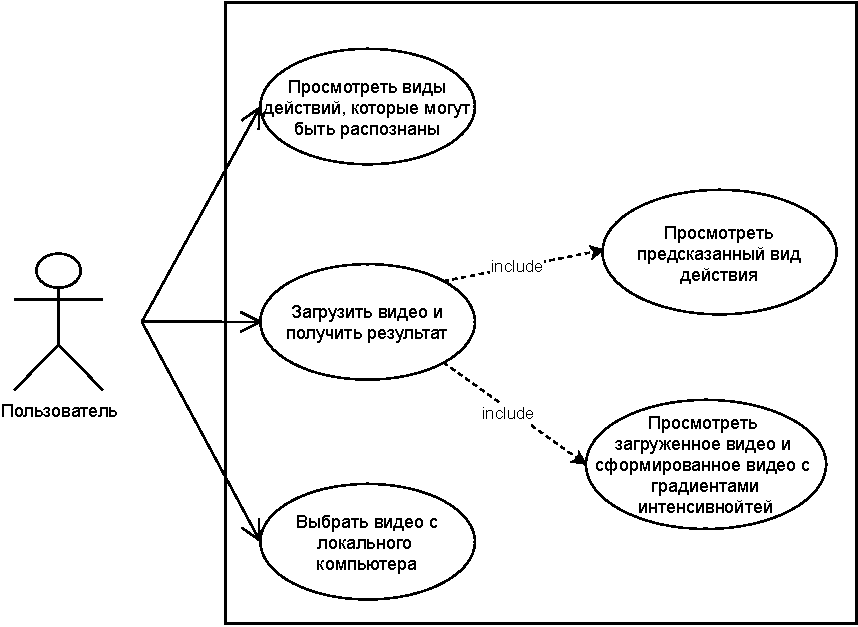
\includegraphics[ scale=0.97]{./img/uml.pdf}
		\caption{UML диаграмма вариантов использования разработанного ПО}  
		\label{fig:xray1}
	\end{center}
\end{figure}
\clearpage
\subsection*{Структура разработанного ПО}

ПО было поделено на следующие основные модули.

\begin{itemize}
	\item[---]  Предобработка данных.
	\item[---]  Формирование дескрипторов видео.
	\item[---]  Обучение модели.
	\item[---]  Классификатор видов действий.
	\item[---]  Графический интерфейс.
\end{itemize}


\subsection{Модуль предобработки данных}
Исходный набор данных содержит видеоролики различного размера кадра, в среднем длительностью 10 секунд. Для получения дескриптора видео, оно должно пройти следующие этапы предобработки:

\begin{itemize}
	\item[---]  разделение видео на кадры;
	\item[---]  обрезание кадра по области, в которой находится человек;
	\item[---]  изменение размера кадра на кратное 16;
	\item[---]  получение черно-белого кадра.
\end{itemize}


На рисунке 3.2 представлен пример преодобработки видео.

\begin{figure}[h]
	\begin{center}
		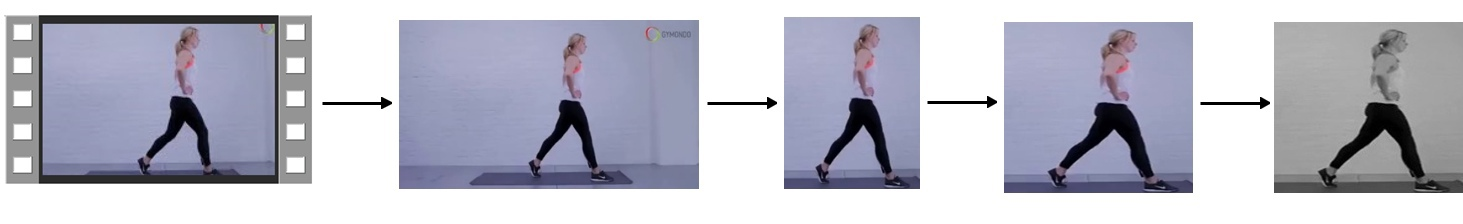
\includegraphics[ scale=0.3]{./img/obr.jpg}
		\caption{Предобработка данных}  
		\label{fig:xray1}
	\end{center}
\end{figure}



На этапе получение кадров использовалась библиотека OpenCV для чтения видео. Для каждого видео вычислялся его fsp и формировался массив длительностей каждого кадра. Далее в цикле для каждого кадра вычислялось его время от начала видео и в случае если время было меньше длительности самого видео, кадр сохранялся.

Для определения области кадра, в которой находится человек был использован метод библиотеки OpenCV, который называется selectROI. С помощью этого метода можно вручную выбрать область изображения, представляющую интерес, путем выделения области на изображении. После этого координаты ограничивающего прямоугольника сохраняются и все последующие кадры обрезаются по полученным координатам. На листинге 3.1 представлена функция обрезания кадра.
\includelisting
{man.py} % Имя файла с расширением (файл должен быть расположен в директории inc/lst/)
{Обрезание кадра} % Подпись листинга

Преобразование размера и цвета кадра происходило с помощью методов библиотеки OpenCV resize и cvtColor.



\subsection{Модуль формирования дескрипторов}
Дескриптор видео формируется на основе кадров видео прошедших этап предобработки и представляет собой массив, элементом которого является дескриптор кадра (массив чисел с плавающей точкой). Для каждого видео дескриптор формируется по 25 кадрам, так как за этот промежуток происходит одно или пару повторяющихся действий и этого достаточно для обучения модели.

В случае формирования дескриптора для обучения в начало массива дескриптора кадра вставляется метка, соответствующая данному типу действия. Формирование дескрипторов производилось многопоточно (10 потоков) и в результате дескрипторы каждого класса действий были сохранены в файлы.
На листинге 3.2 представлена функция формирования дескрипторов каждого класса для их сохранения.

\includelisting
{save.py} % Имя файла с расширением (файл должен быть расположен в директории inc/lst/)
{Сохранение дескрипторов тренировочной выборки} % Подпись листинга
\subsection{Модуль обучения модели}

Обучение модели проводилось с помощью встроенного классификатора случайного леса библиотеки Scikit-learn RandomForestClassifaer. 
\clearpage

%На листинге представлен прототип функции RandomForestClassifaer.

%\includelisting
%{prototype.py} % Имя файла с расширением (файл должен быть расположен в директории inc/lst/)
%{Прототип функции RandomForestClassifaer} % Подпись листинга

Для обучения модели необходимо было определить параметры, при которых модель обеспечивает наилучшую точность, это можно было сделать используя поиск по сетке. Поиск по сетке (Grid Search) -- это алгоритм оптимизации, который позволяет определить лучшие параметры для оптимизации проблемы из списка вариантов, который задан, тем самым автоматизируя метод «проб и ошибок». На листинге 3.3 представлена реализация поиска по сетке.

\includelisting
{search.py} % Имя файла с расширением (файл должен быть расположен в директории inc/lst/)
{Поиск по сетке} % Подпись листинга

Был проведен поиск по сетке в результате, которого в качестве оптимальных параметров классификатора были определены следующие значения: bootstrap = false, criterion = entropy, n\_estimators = 1000.

Модель способна распознавать действия для каждого кадра видео и с помощью функции mode() определяется наиболее часто встречающееся метка действия среди 25 кадров, действие соответствующие этой метки возвращается как результат распознавания типа действия на видео.

 Перед обучением производится чтение дескрипторов из файлов, полученных в результате обработки тренировочного набора данных, и их объединение. Также происходит разделение полученного массива данных на дескрипторы и соответствующие им метки. Массив меток и дескрипторов передаются в функцию обучения модели, и уже обученная модель сохраняется в файл.

% На листинге представлена функция обучения модели распознавания спортивных действий.

%\includelisting
%{train.py} % Имя файла с расширением (файл должен быть расположен в директории inc/lst/)
%{Обучение модели} % Подпись листинга


\section{Тестирование модели}\label{test}
На тестовом наборе данных, составляющем 30\% исходного набора, проводилось тестирование модели в результате которого была сформирована матрица ошибок. Так как в каждом классе содержалось разное количество видео, для тестирования каждого класса было выбрано 30\% от соответствующего объема видеороликов этого класса. 

Матрица ошибок -- это показатель успешности классификации, где классов два или более. Она представляет собой таблицу с 4 различными комбинациями сочетаний, прогнозируемых и фактических значений.

Матрица ошибок формировалась для многоклассовой классификации из 10 классов. В алгоритме кросс-валидации класс, который представляет для нас интерес, называется «положительным», а оставшиеся – «отрицательными».

Поэтому для каждого объекта в выборке возможно 4 ситуации:

\begin{itemize}
	\item[---]  предсказана положительная метка и это верно. Такие объекты относятся к истинно-положительной (TP, true positive) группе. Истинно потому что предсказание верное, а положительный, потому что предсказываем объект  положительного класса;
	\item[---] предсказана положительная метка, но предсказание ошибочно – ложно-положительный (FP, false positive). Ложное, потому что предсказание было неправильным;
	\item[---]  предсказана отрицательная метка и это верно -- истинно-отрицательный (TN, true negative);
	\item[---]  предсказана отрицательная метка, но предсказание ошибочно -- ложно-отрицательный (FN, false negative).
\end{itemize}

Так в результате %производился подсчет количетва случаев каждой из этих ситуаций и%
сформирована матрица ошибок, где на главной диагонали показано количество объектов положительного класса (TP), которые верно предсказаны, а на пересечение видов действий количество ошибочных предсказаний (FN). В качестве объекта предсказания принимается кадр видео. На рисунке 3.3 представлена матрица ошибок модели распознавания спортивных действий человека.

\begin{figure}[h]
	\begin{center}
		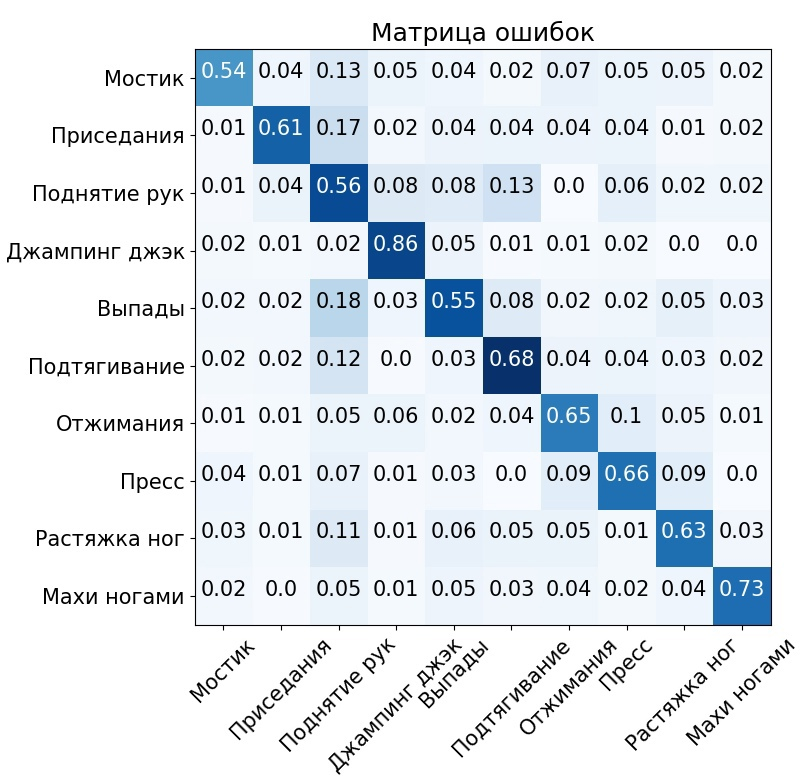
\includegraphics[ scale=0.5]{./img/matrix1.jpg}
		\caption{Матрица ошибок}  
		\label{fig:xray1}
	\end{center}
\end{figure}
 

\section{Пользовательский интерфейс}

Интерфейс был реализован с помощью веб-фреймворка Flask. На сайте пользователю доступно две страницы. На странице справка описаны характеристики видео, которое нужно загрузить для успешного распознавания, а также все виды действий, которые подлежат распознаванию с видео примерами. На рисунке 3.4 представлена страница со справочной информацией.
\clearpage

\begin{figure}[h]
	\begin{center}
		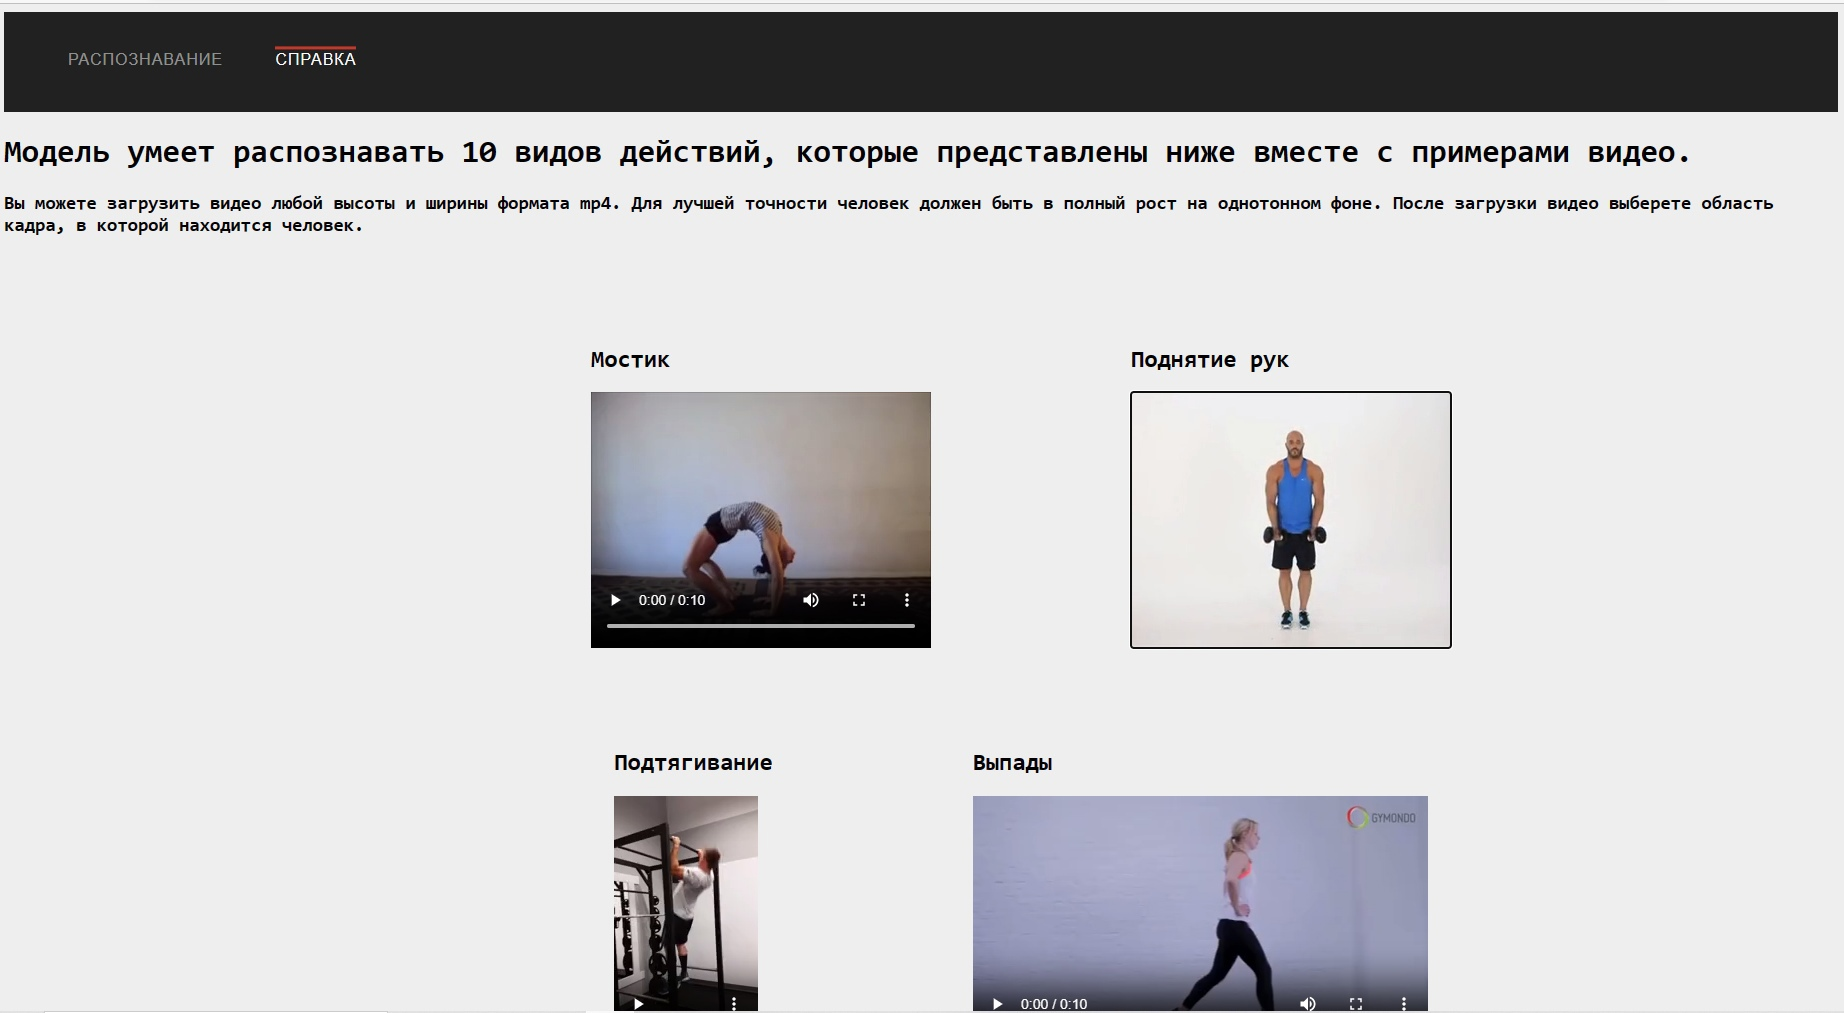
\includegraphics[ scale=0.25]{./img/info.jpg}
		\caption{Страница справка}  
		\label{fig:xray1}
	\end{center}
\end{figure}

На главной странице есть форма с помощью, которой пользователь может загрузить видео для предсказания вида действия со своего локального компьютера, нажав кнопку выбрать файл. На рисунке 3.5 представлена главная страница сайта.
\newpage
\begin{figure}[h]
	\begin{center}
		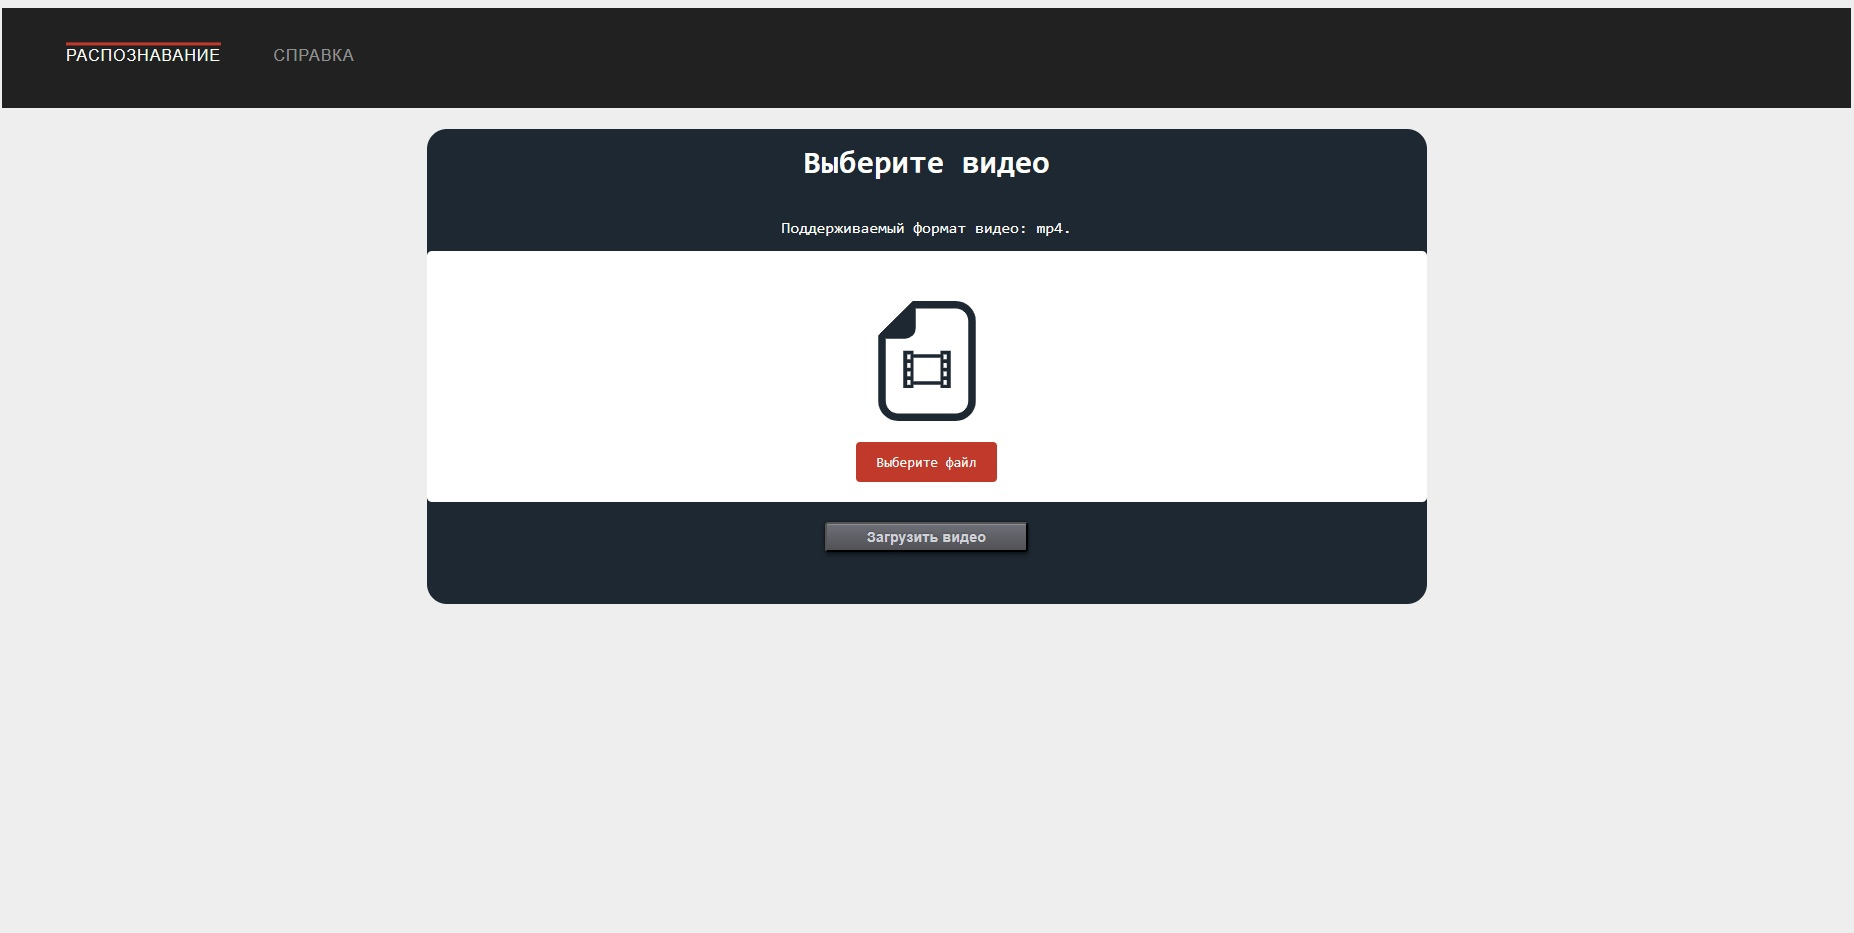
\includegraphics[ scale=0.25]{./img/main.jpg}
		\caption{Главная страница}  
		\label{fig:xray1}
	\end{center}
\end{figure}

При нажатии кнопки выбрать файл открывается диалоговое окно, в котором пользователь должен выбрать нужный ему видеоролик. Далее нажать кнопку загрузить видео и ожидать результат предобработки и предсказания вида действия. На рисунке 3.6 представлен процесс загрузки видео.

\begin{figure}[h]
	\begin{center}
		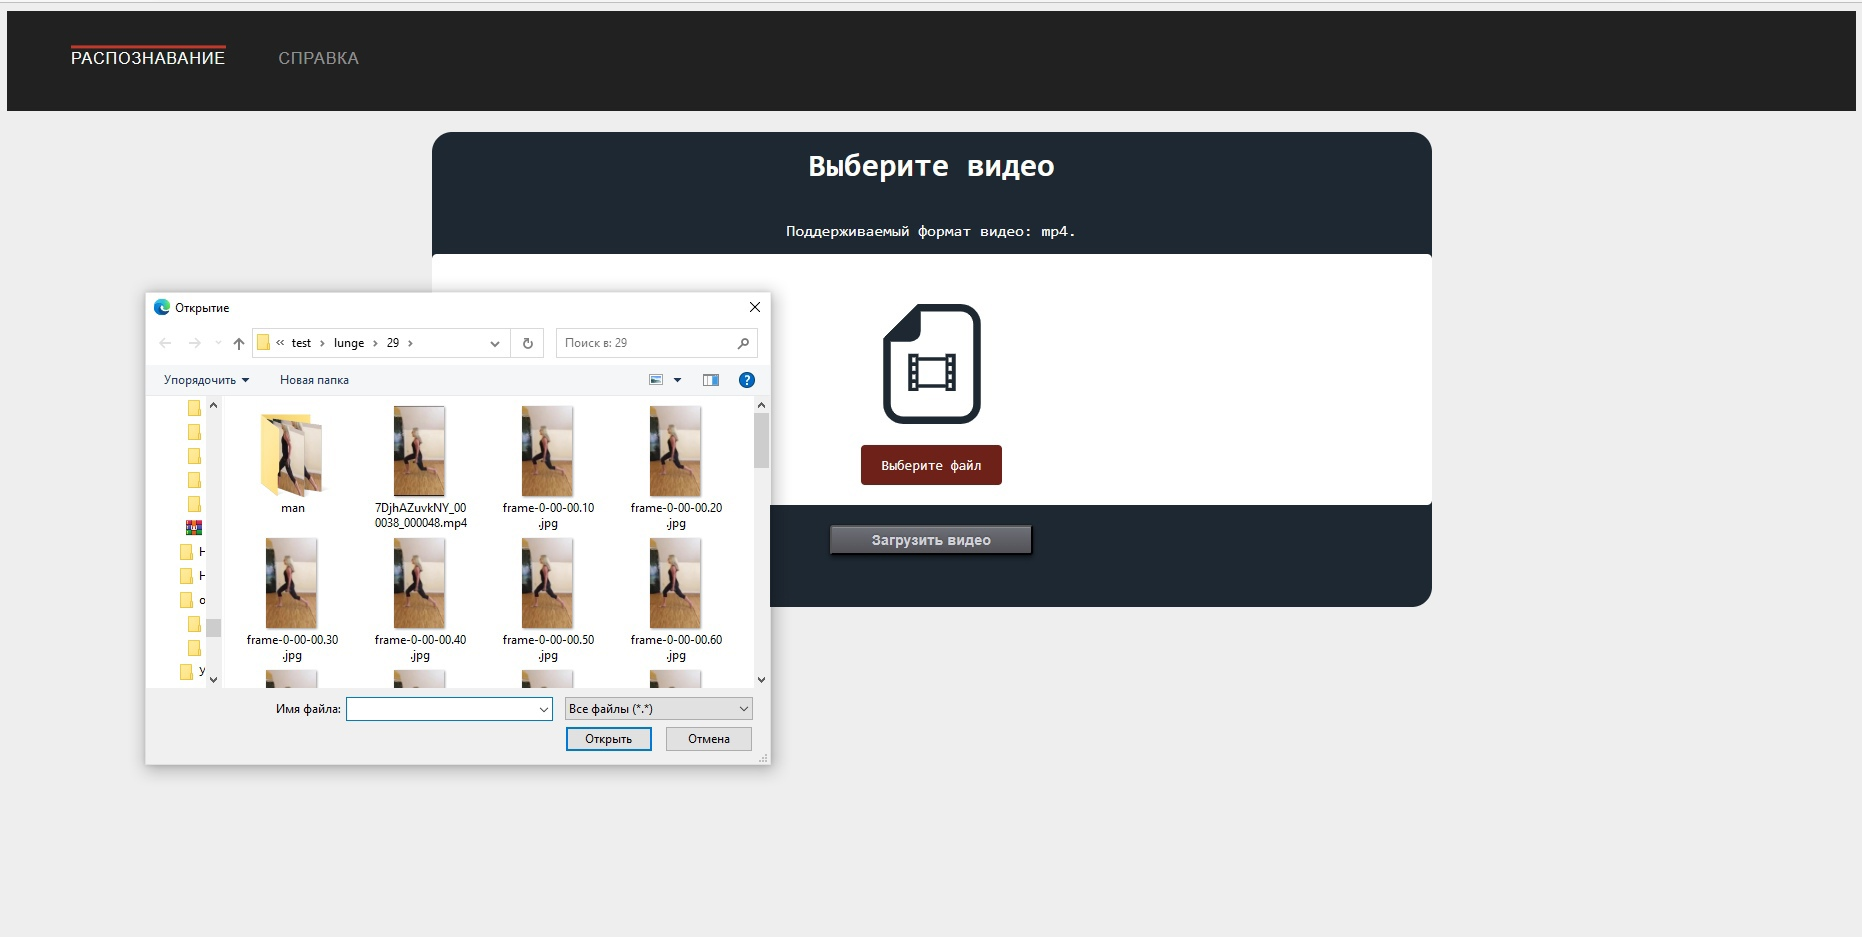
\includegraphics[ scale=0.23]{./img/upload.jpg}
		\caption{Загрузка видео}  
		\label{fig:xray1}
	\end{center}
\end{figure}
\clearpage
В результате на странице пользователю представлено исходное видео и предсказанный вид действия. Также для визуального представления помимо основного видео формируется видео из кадров, на которых изображены направления интенсивности, используемые для формирования дескриптора. На рисунке 3.7 представлен результат работы ПО.
\begin{figure}[h]
	\begin{center}
		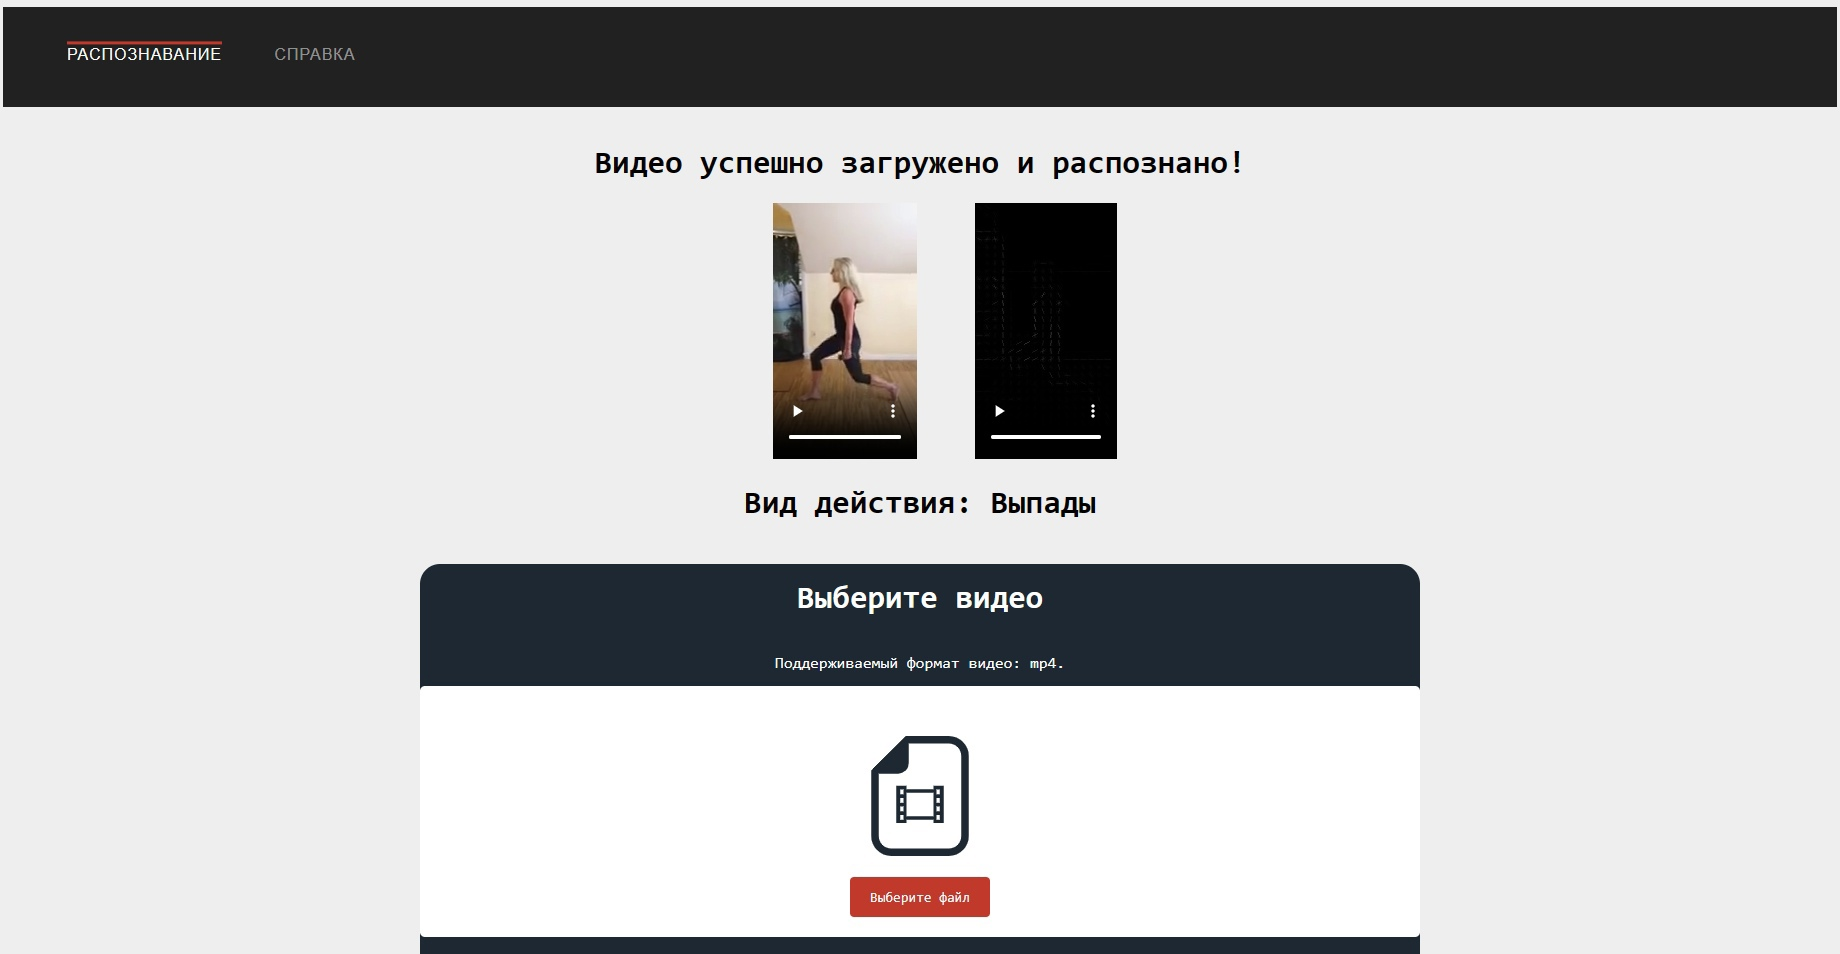
\includegraphics[ scale=0.25]{./img/result.jpg}
		\caption{Результат распознавания}  
		\label{fig:xray1}
	\end{center}
\end{figure}

\section*{Вывод}
В данном разделе произведен выбор средств программной реализации метода, описан формат входных и выходных данных ПО. Приведены детали реализации программных компонентов, предоставлены результаты тестирование разработанного метода, описано взаимодействие пользователя с интерфейсом ПО, реализующим метод. 